\FloatBarrier
\subsection{Poker Flat ISR (PFISR)}\label{sec:fuspfisr}
PFISR produces several low-level data products including the complex analog-to-digital converter voltage samples.
At the time, access to the large files containing low-level PFISR data is by request, with radar data accumulating at $\sim \unit[1.5]{MB/s}$ during a typical experiment.
% data: Apr 14 2013  (468530486 + 224263860 + 224263860 + 187839490) bytes / 729 seconds = 1.516 MByte/sec
Madrigal PFISR high-level data products have integration times $\sim \unit[2]{min}$ versus \unit[10..100]{ms} cadence of the low-level PFISR data.
Long integration time is necessary for plasma parameter estimation since incoherent returns from the ionospheric volume target provide return signals far too weak to characterize from a single pulse.
An autocorrelation function (ACF) is built up from the incoherent electron and ion scatterers over tens of seconds.
Taking the Fourier transform of the ACF the power spectral density (PSD) is obtained, with a notional PSD from a quiet ionosphere shown in Figure~\ref{fig:isrmorph}(a).
An ACF fitting algorithm provides estimates of electron number density, electron and ion temperature and ion velocity.

These plasma parameter estimates break down when turbulent plasma leads to a breakdown in the parameter fitter, which expects PSDs having morphology similar to Figure~\ref{fig:isrmorph}(a).
Strong Langmuir turbulence \citep{akbari2012} leads to ISR spectrum like that depicted in Figure~\ref{fig:isrmorph}(b).
\begin{figure}\centering
    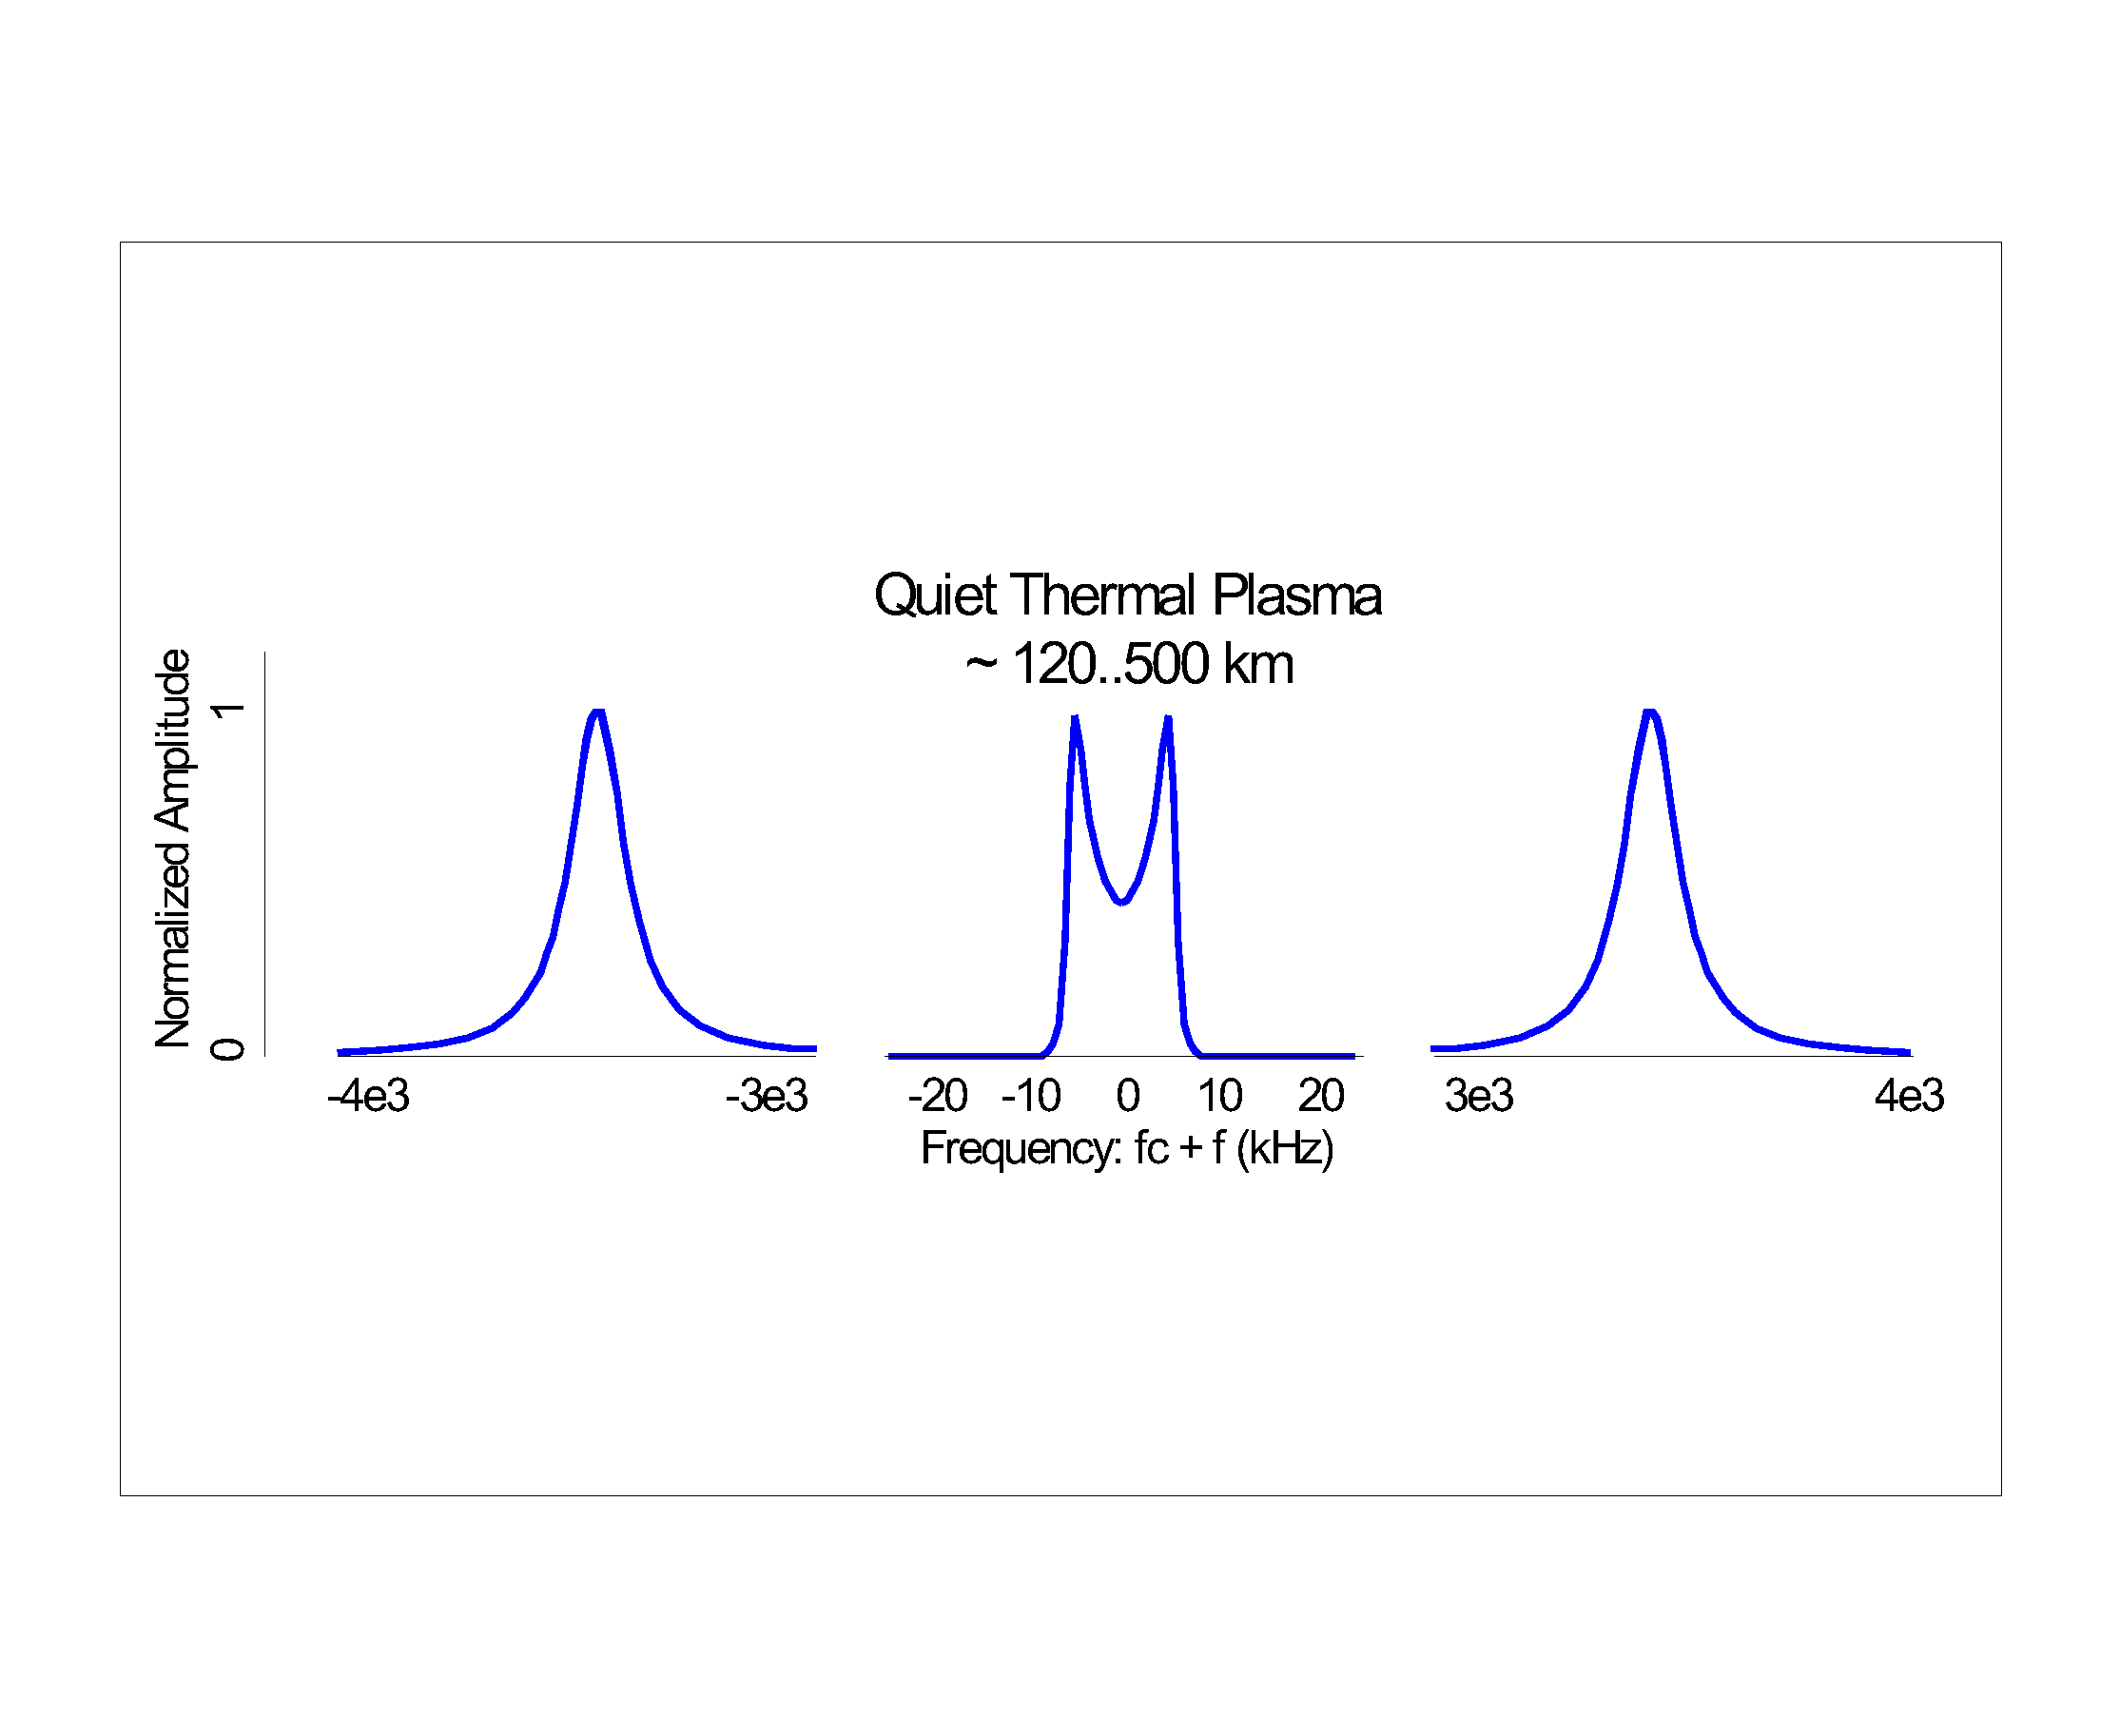
\includegraphics[width=0.8\columnwidth,trim=80 260 100 280,clip]{gfx/isr_thermal}

    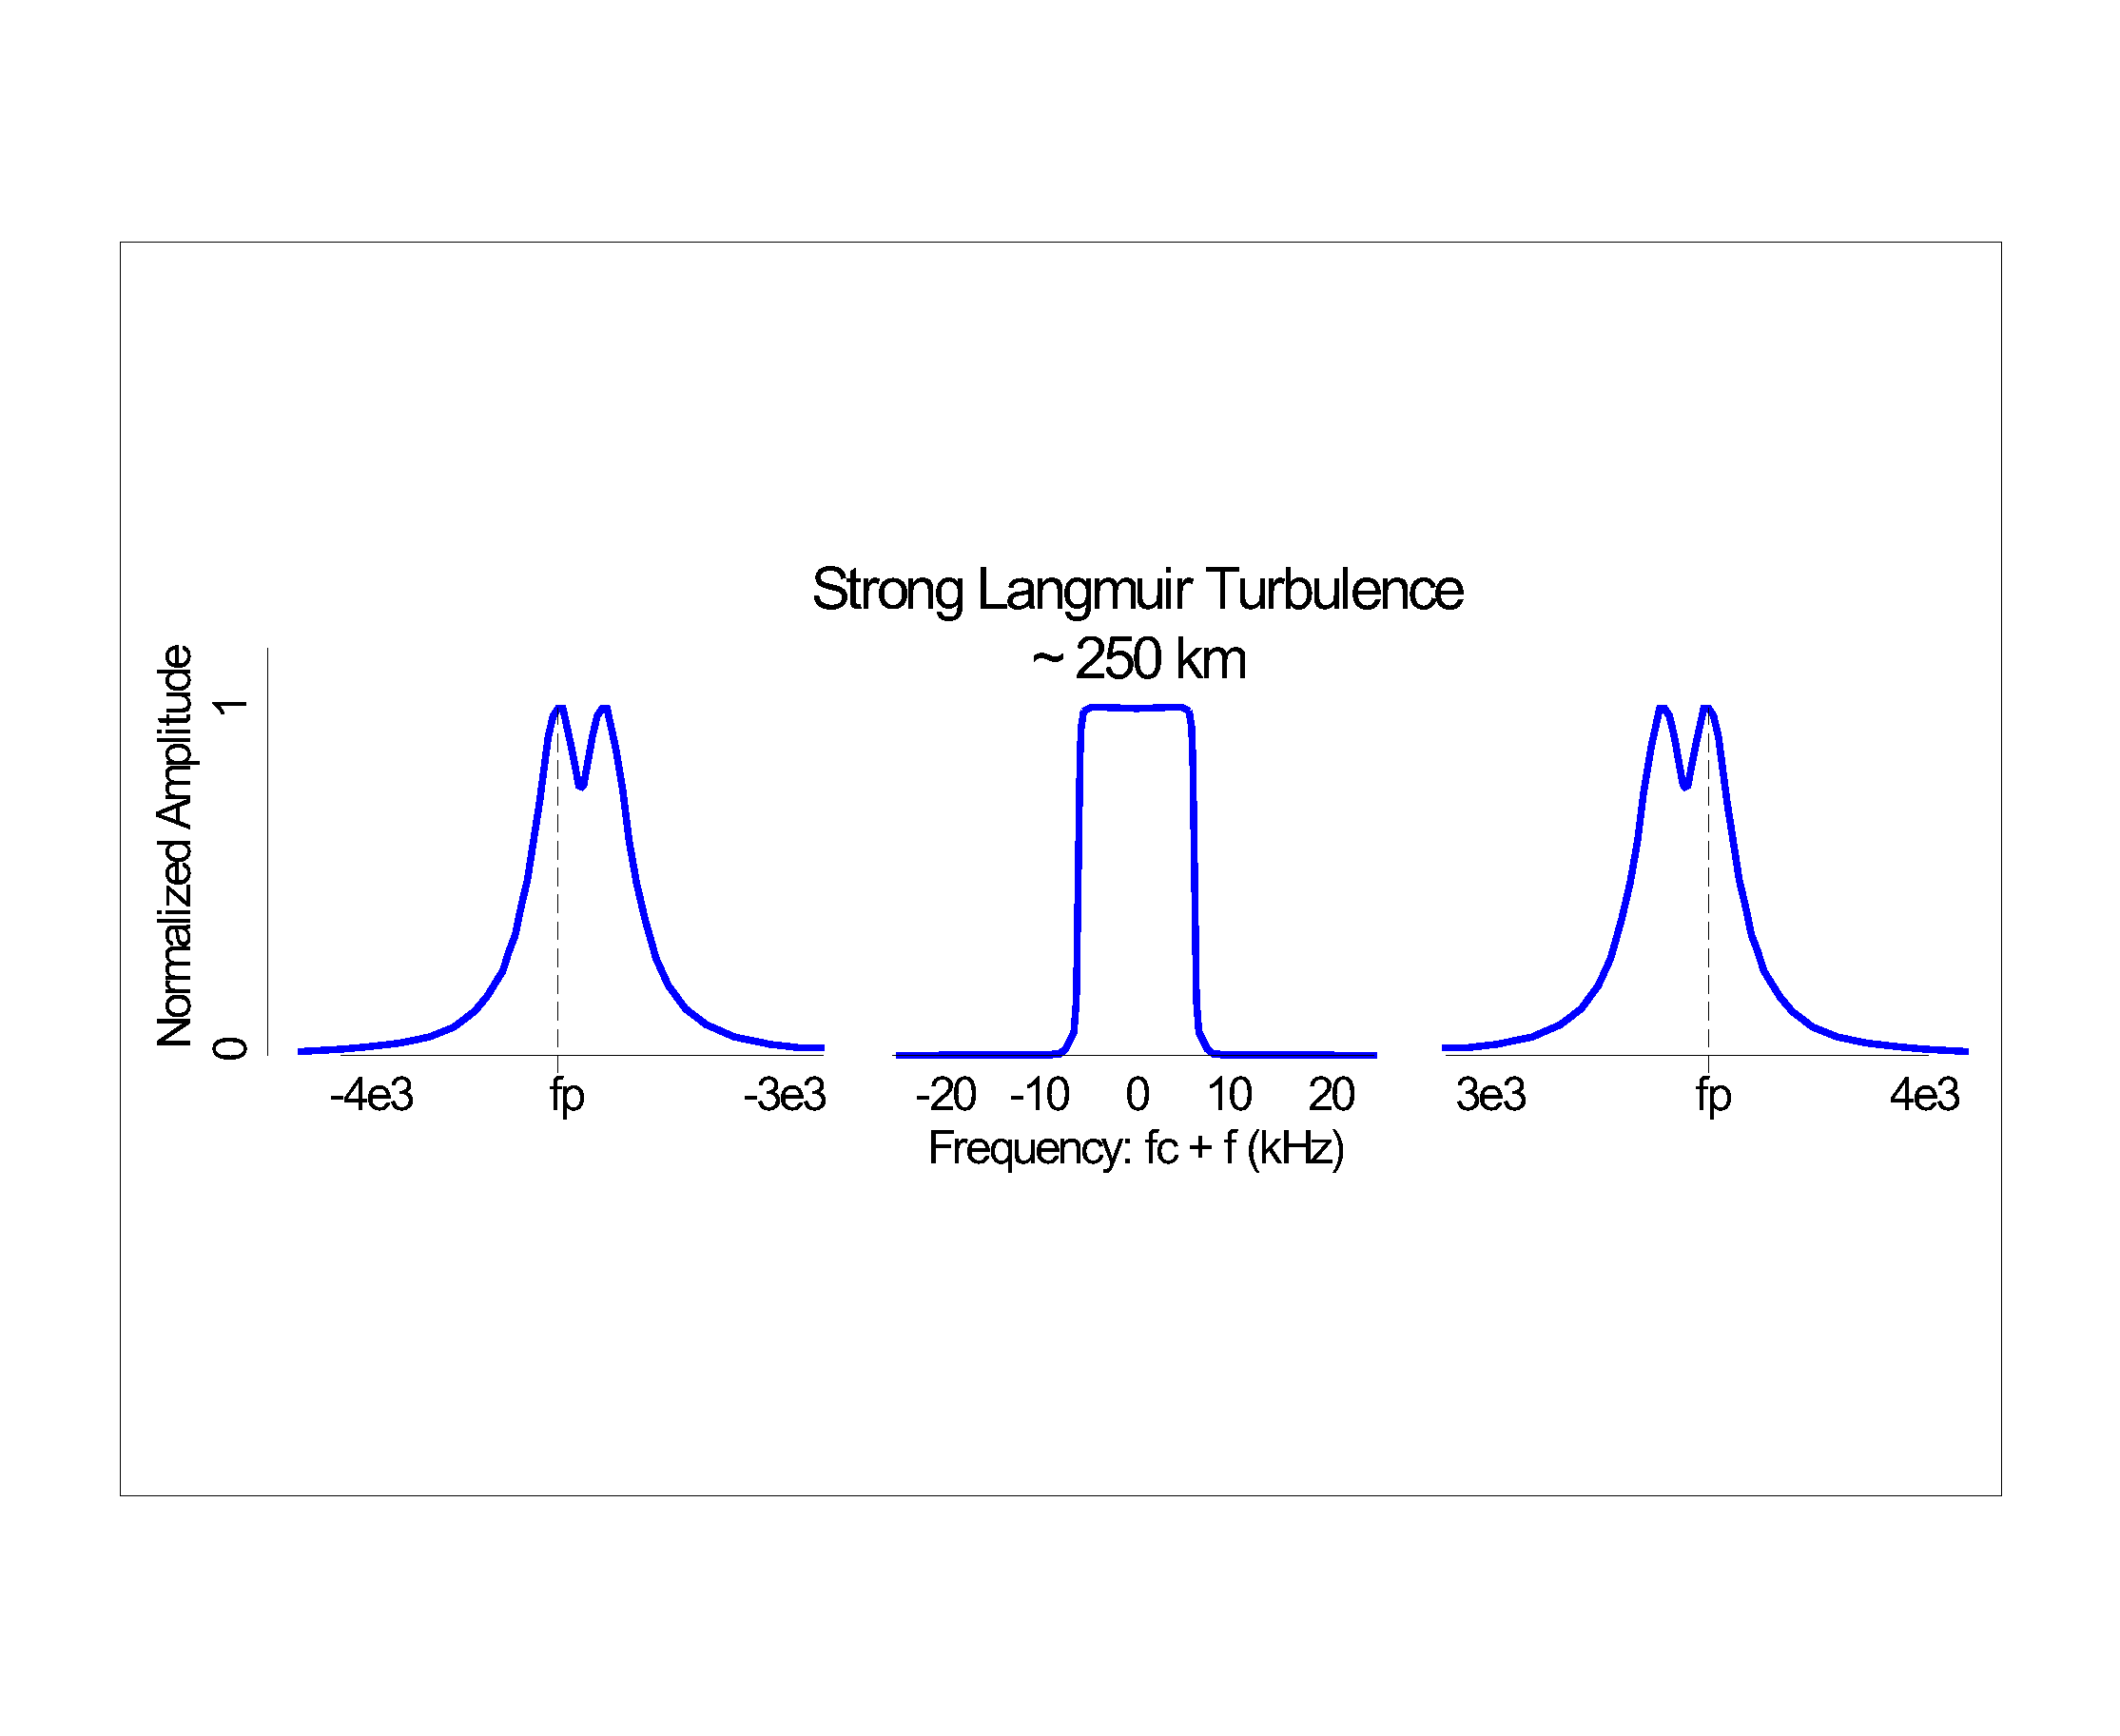
\includegraphics[width=0.8\columnwidth,trim=80 260 100 270,clip]{gfx/isr_slt}

    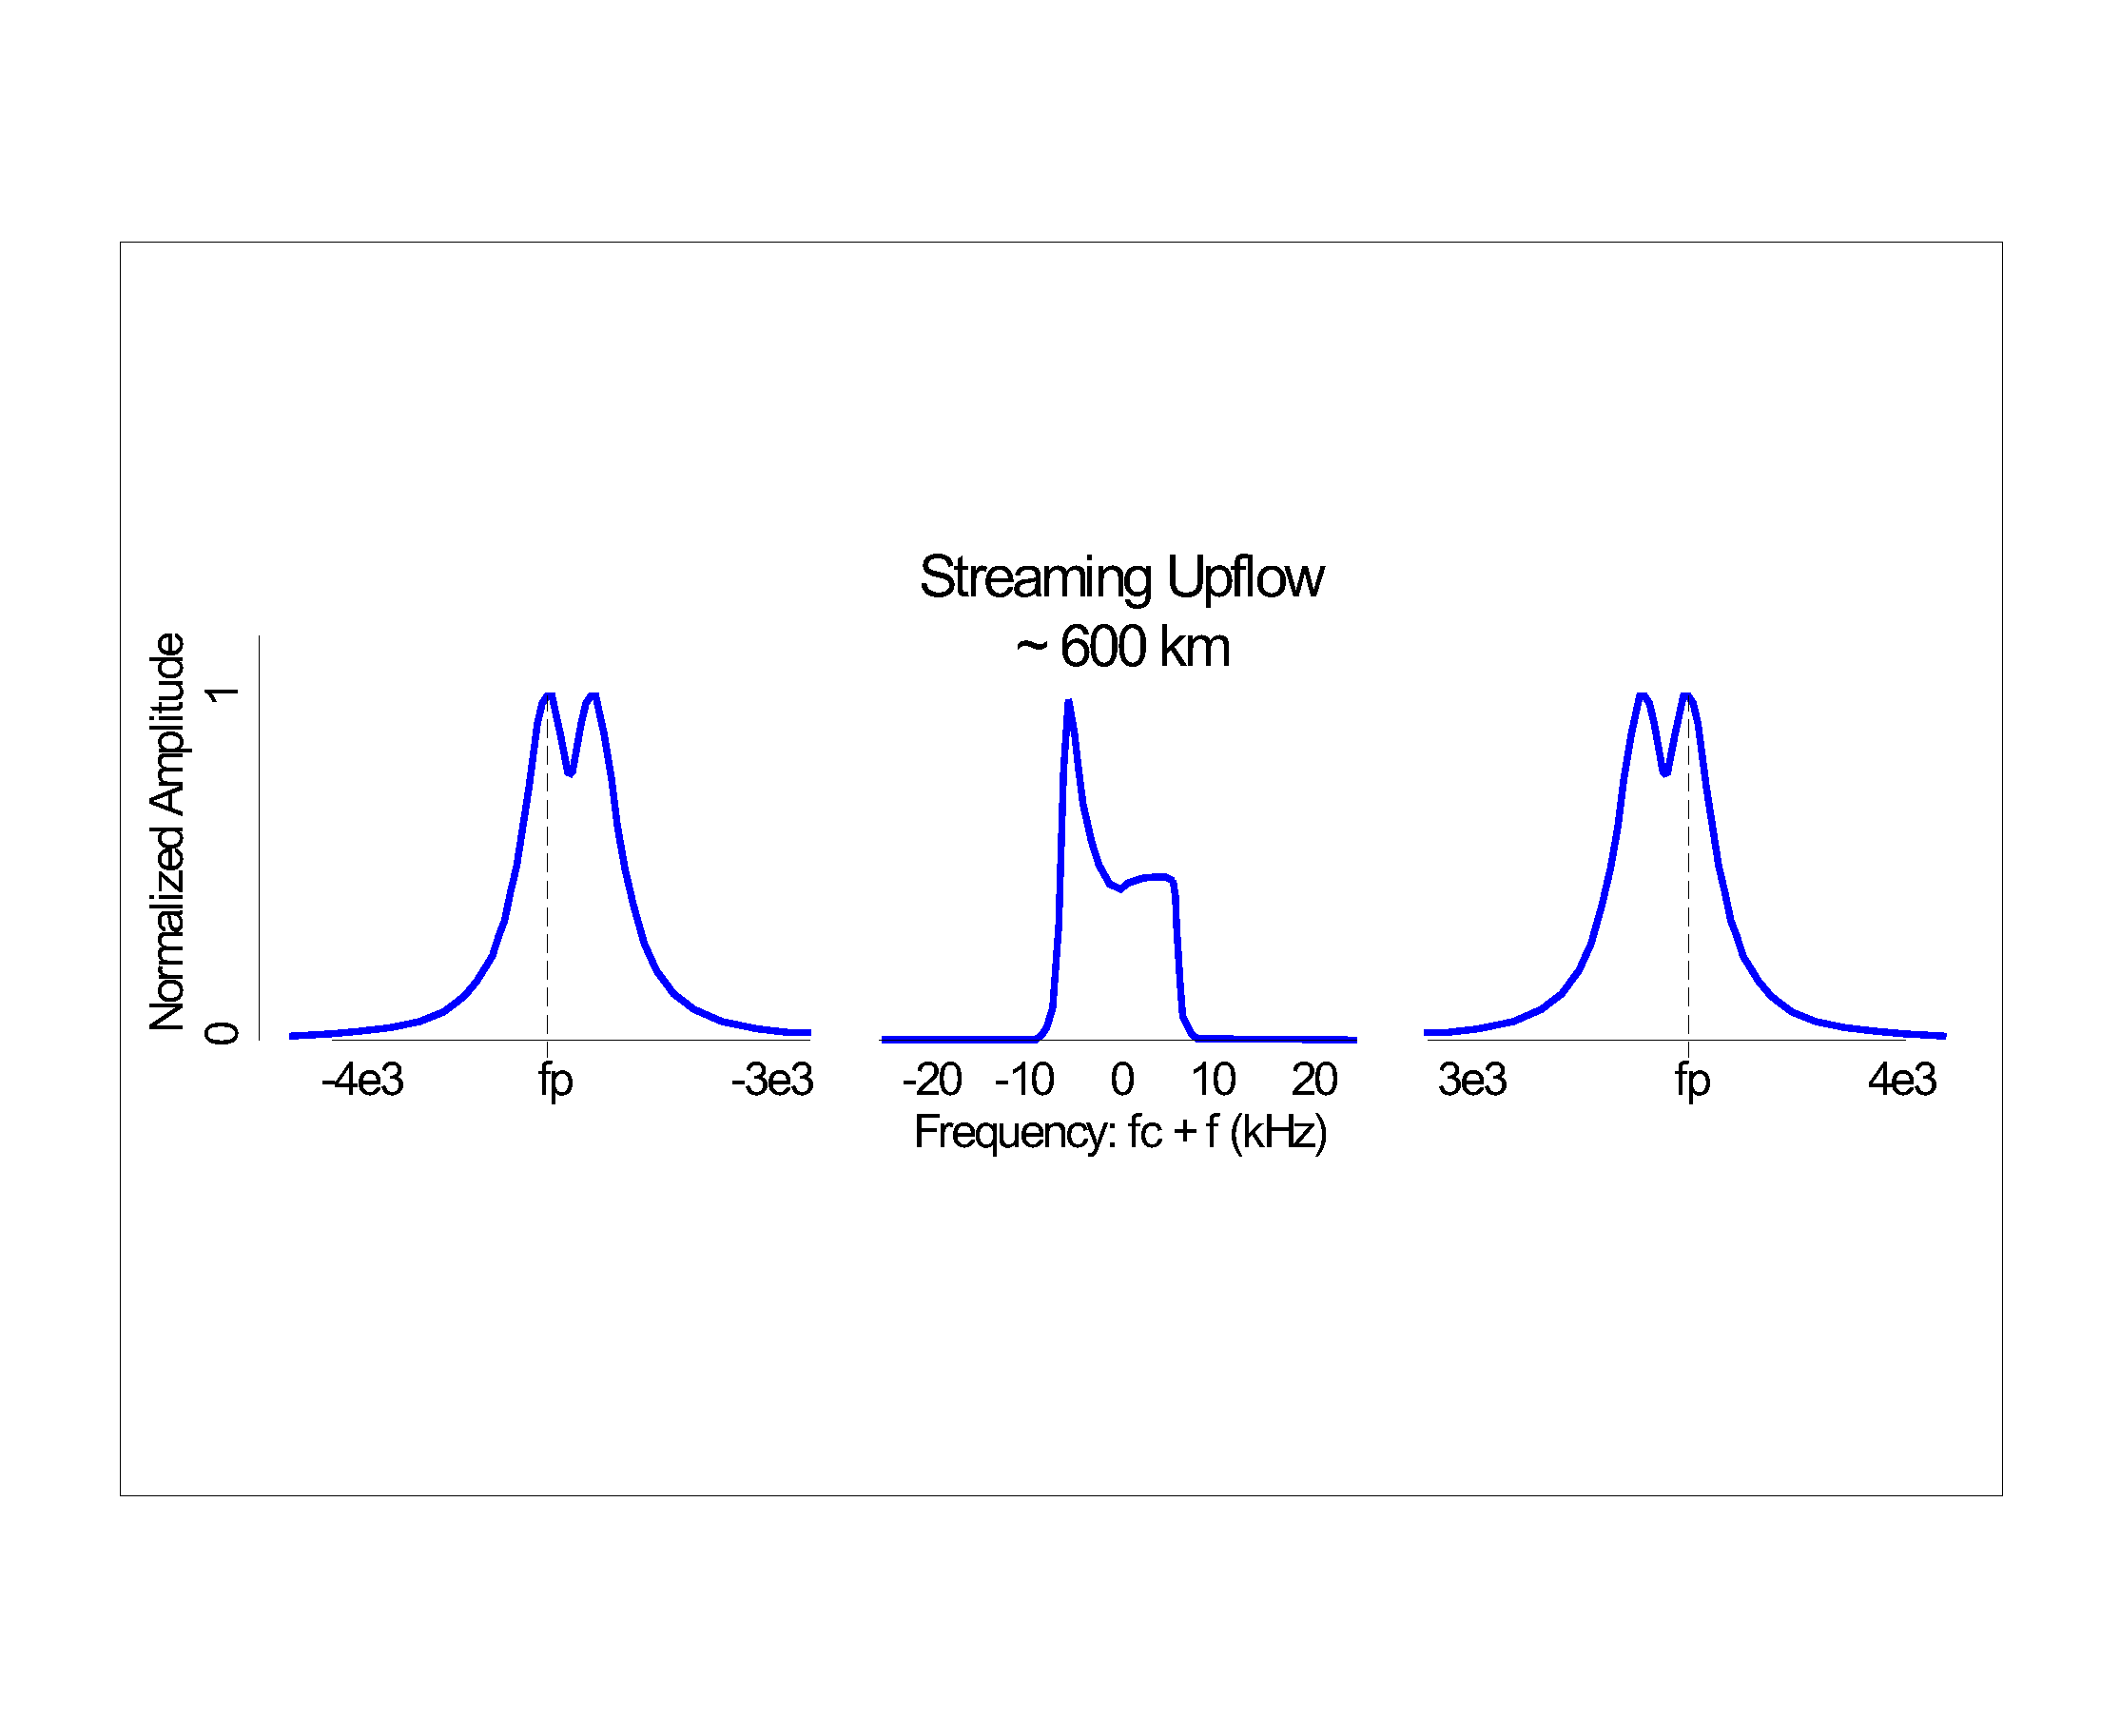
\includegraphics[width=0.8\columnwidth,trim=80 260 100 270,clip]{gfx/isr_streamupflow}
    \caption{(a) Notional PFISR spectrum for quiet ionospheric conditions. 
    	(b) Notional PFISR spectrum under strong Langmuir turbulence. 
    	(c) Notional PFISR spectrum with streaming upflowing plasma.}
    \label{fig:isrmorph}
\end{figure}
Streaming upflows lead to ISR spectrum similar to the depiction in Figure~\ref{fig:isrmorph}(c).
The ISR fitter algorithm used in plasma parameter estimation assumes a single-Maxwellian distribution, which breaks down under turbulent conditions, leading to non-physical plasma parameter estimates.
Alfvénic aurora associated with this Langmuir turbulence leaves fingerprints in the auroral morphology HiST was designed to observe.

The PFISR complex vector $\mathbf{I}+j\mathbf{Q}$ sampled time series is obtained with revisit time as fast as \unit[75]{ms} \citep{akbari2012} for five-beam pattern experiments and may be pushed at least to \unit[19]{ms} \citep{michell2009} for single-beam position experiments.
For future measurements, new ISR plasma line receiver techniques \citep{vierinen2016} reduce plasma line sampling cadence to about \unit[200]{ms}.
Table~\ref{tab:cadence} summarizes the time sampling capability of PFISR.
\begin{table}\centering
    \caption{Instrument sample rates vs. resolution used in experiments.}\label{tab:cadence}
    \begin{tabular}{llll}
        \toprule
        Instrument Measurement Mode & Resolution & Cadence [ms] & Date\\
        \midrule
        PFISR ion line long pulse & five beams    & 75   & 2011-03-01 \\
        PFISR plasma line long pulse & five beams & 6000 &  \\
        Andor Neo sCMOS camera & $1280 \times 1080$  & 20 &  \\
        \midrule
        PFISR ion line long pulse & 23 beams      & 234  & 2013-04-14 \\
        PFISR plasma line long pulse & 23 beams & 14000 &  \\
        Andor iXon EMCCD camera & $512 \times 512$ & 20 & \\
        \bottomrule
    \end{tabular}
\end{table}

Radar receive power for a beam-filling target may be described as
\begin{equation}
%P_r = K\frac{\tau_p P_t}{r^2}G_t G_r n_e \sigma
P_r = (F G_0) P_t L n_e \sigma c \tau \lambda^2 (64 \pi^2 r^2)^{-1} \textrm{[watts]}
\end{equation}
where $P_r$ is power received at the antenna terminals, $F$ is the antenna taper factor accounting for non-boxcar shape of beam, taken as 0.76 in \citet{evans1969}, $G_0$ is boresight antenna gain, $P_t$ is the power transmitted at the antenna terminals, $L$ is radar system losses, $\tau$ is the radar pulse length and $r$ is the one-way slant range to the measured range gate (alternatively called voxel or resolution cell).
The cross section of the beam-filling target is \citep{nicolls2015,evans1969}
\begin{equation}
\sigma = \frac{\sigma_e}{(1+\alpha^2)(1+\frac{T_e}{T_i} + \alpha^2)}
\end{equation}
where $\alpha = 4\pi \lambda_D / \lambda$, the radar cross section of an electron is 
\begin{equation}
\sigma_e = 4 \pi(r_e \sin \psi)^2
\end{equation}
the electron radius is
\begin{equation}
r_e = \frac{e^2}{\varepsilon_0 m_e c^2}
\end{equation}
and $\psi=\pi/2$ for a backscattered electron \citep{evans1969}.
For computing SNR, the noise power is
\begin{equation}
P_n = k_B T_s B
\end{equation}
where $T_s$ is system temperature.
The ISR PSD shape is a function involving many terms, and the reader is referred to \citet{evans1969} equations (18-21) for the specifics.


PFISR ion-line PSD is obtained by taking the Fourier transform of the autocorrelation function.
The ion line spectra are typically observed as two equal-amplitude frequency-smeared impulses symmetric about the radar center frequency.
Typical Doppler bandwidth is less than \unit[25]{kHz} for the \unit[450]{MHz} AMISR.
PFISR plasma-line spectra are shifted several MHz up and down from the radar center frequency, so a slice of the receiver spectrum is extracted where the plasma lines are expected to occur to conserve data and storage resources.
Under quiet and inverted-V auroral conditions, the ISR ion-line spectrum assumptions made by the fitter are fulfilled.
Using assumptions on atmospheric composition (species and density) vs. altitude, an least squares fit of the ion-line PSD is made to estimate the plasma parameters $N_e, T_e, T_i, V_i$.
Further consideration of the fitting of plasma parameters to the ion-line spectrum is given in \citet{swobodathesis}.


A summing-over-altitude technique is useful in both the ion line and plasma line data as a method to draw out weaker coherent returns not otherwise visible.
We integrate $P_r$ in the NEIAL altitude range of roughly \unit[200..400]{km} and plot this integrated measurement as a time series with a representative NEIAL event in Figure~\ref{fig:shedintion}.
\begin{figure}
    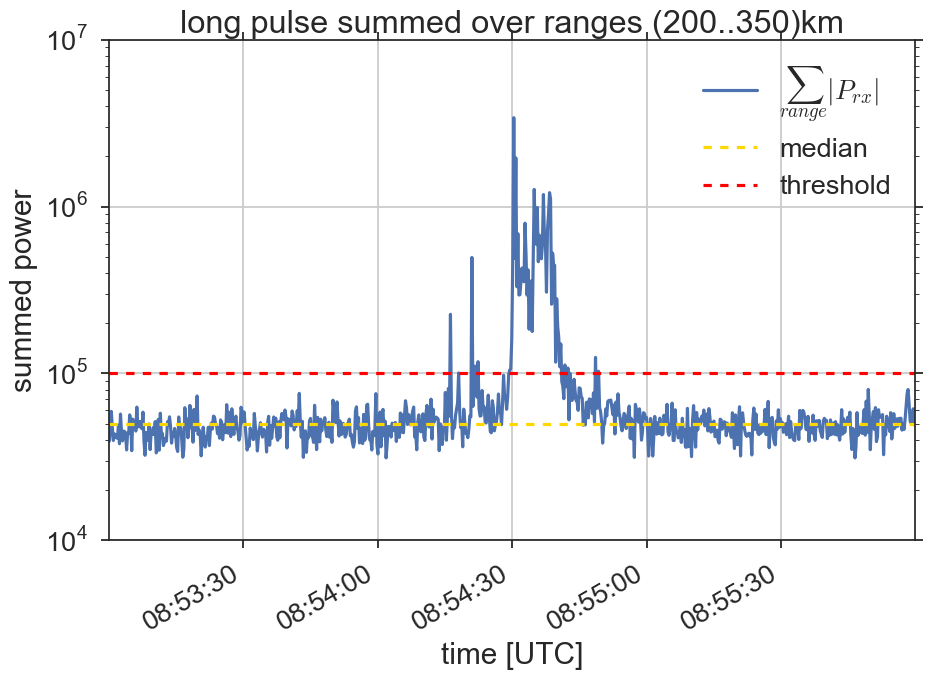
\includegraphics[width=0.9\columnwidth]{gfx/2013-04-14T0854/summedAlt2013-04-14T08-54}
    \caption{Receive power of Figure~\ref{fig:20130414T0854a}(e) integrated over \unit[200..350]{km}. 
        Observe turbulence perturbation from approximately 8:54-8:55~UT.}
    \label{fig:shedintion}
\end{figure}
Considering the large amount of raw data collected each day, a method of automated turbulence detection is quite useful, particularly during daylight hours when auroral video is not available.
Cell-median CFAR is the method used in this work.
\citet{schlatter2014} used image processing techniques to further restrict ``matching'' events. 
In contrast, the goal in this work was to achieve high sensitivity and manually filter out spurious events such as satellites.
Most of the time turbulence does not occur, so we can use the median of the last $N$ measurements and set a threshold based on a constant $K$ factor above this rolling median $\widetilde{M}$.
Using Figure~\ref{fig:shedintion} as an example, suppose the rolling median is 50,000.
We can decide detection by
\begin{equation}\label{eq:cfarsum}
S \gtrless K\cdot\widetilde{M}
\end{equation}
based on summed power $S$ vs $K=2.0$ as the threshold factor in this example.
